(CHECK Version/Carlo 21.11)\\
In diesem Kapitel werden Werkzeuge vorgestellt, mit denen Budgets mit Alarmen erstellt werden, diese informieren, wenn ein bestimmter Prozentsatz des festgelegten Budgets überschritten wurde. Die Erstellung von Budgets trägt zu einer besseren Planung-/Prognose- und Kostenkontrolle. ZITAT?
Die Einstellung von Alarmen für relevante Ereignisse wie im Fall einer Budgetüberschreitung oder dem Start einer Instanz[IST GUT WEIL/TRÄG ZU...BEI].

Darüber hinaus ist es mit Werkzeugen wie CloudWatch möglich, die Abschaltung bestimmter Dienste zu automatisieren, wenn eine Budgetschwelle überschritten wurde. Diese Maßnahmen werden in dem Kapitel über die Optimierung behandelt.

Durch die Verwendung von Tags ist es möglich, die Ressourcen nach Kriterien wie Region, Umgebung, Projekt, Art der Ressource usw. zu visualisieren, dies %es
ermöglicht, Kosten auf den von der Organisation festgelegten Ebenen zu verfolgen. 
[DIAGRAMM: BUDGET PRO ABTEILUNG]\\
Es könnte zum Beispiel ein Szenario entstehen, in dem eine Abteilung innerhalb der Organisation mehr Kosten verursacht als andere. In erster Linie ist dies nur bemerkenswert anhand eines Anstiegs der von Amazon generierten Rechnung, aber um den Grund für diesen Anstieg genauer zu verstehen, muss ihre Ursache untersucht werden. Werkzeuge wie Cost-Explorer machen diese Art von Analyse möglich.

TRUSTED ADVISOR(Einleitung)??
%Zu diesem Zweck werden Werkzeuge vorgestellt, die die Überwachung aktiver Ressourcen ermöglichen.
%Welche Kosten sind mit der Nutzung dieser Werkzeuge verbunden?
%Es sollte gezeigt werden, die Arten/Kategorien von Kunden, die kostenlosen Zugang zu diesen Werkzeuge haben?
%WAS MIT AWS Budgets? AWS Bill and cost Man.?

\subsection{AWS CloudWatch}
%https://aws.amazon.com/de/cloudwatch/pricing/
%https://docs.aws.amazon.com/AmazonCloudWatch/latest/monitoring/GettingStarted.html

Amazon CloudWatch ermöglicht die Überwachung der Leistung von Resources, auch bei Ressourcen, die über verschiedene Regionen verteilt sind.
CloudWatch sammelt operative Daten für die Verlaufsanalysen und die Entscheidungsfindung in Bezug auf Optimierung und Fehlerbehebung.

CloudWatch beschränkt sich nicht nur darauf, Daten aus der AWS-Umgebung zu empfangen.  Externe CloudWatch fähige? Metriken sind ebenfalls zugelassen und können für eine einheitliche Analyse aggregiert werden.

Eine der Metriken, die mit Amazon CloudWatch überwacht werden kann, ist die CPU-Auslastung von EC2-Instanzen.
Basierend auf einem Prozentsatz der CPU-Auslastung können Alarme?Benachrichtigungen?[WELCHES WORT?] und Aktionen konfiguriert werden
\\
Eine dieser Aktionen ist die automatische Einrichtung neuer Instanzen zur Deckung des Kapazitätsbedarfs
\footnote{\cite{AWS1}, Seite 185}.
Diese Art von Aktionen werden im Kapitel ~\ref{kap_Optimierung} Optimierungsmaßnahmen tiefer behandelt.
\\\\
Im Folgenden werden die grundlegenden Bereiche und Begriffe von CloudWatch erläutert und wie sie zur Überwachung von Informationen über AWS-Ressourcen verwendet werden.
\\\\
\textbf{Metriken} \\
Eine Metrik stellt eine Reihe von Daten über die Leistung einer Ressource in zeitlicher Reihenfolge dar. Standardmäßig werden viele kostenlose Metriken an CloudWatch übermittelt.
\begin{comment}\\
Metriken bleiben wie folgt verfügbar:\\
Auflösung/Zeitraum: \\
1 Minute - 15 Tage\\
5 Minuten - 63 Tage.\\
1 Stunde - 15 Monate
\footnote{\cite{AMZ15}, Wie lange werden die verfügbaren Metriken aufbewahrt?}
\end{comment}
Zum Beispiel kann der Durchschnitt von einer bestimmten API pro Stunde untersucht werden.
Für eine detailliertere Überwachung ist es möglich, benutzerdefinierte Metriken zu konfigurieren, die eine Auflösung von bis zu 1 Sekunde zulassen. Ein praktisches Beispiel für benutzerdefinierte Metriken ist die Messung der Ladezeit einer Website.
[EIN BEISPIEL MIT BEZUG AUF K:OPTIMIERUNG?oder WIESO IST DIE AUFLÖSUNG RELEVANT?]
%\textbf{Logs} \\ BRAUCHE ICH DAS?
\\\\
\textbf{Ereignisse / Events} 
\\
Bei CloudWatch ist ein Ereignis eine Änderung bei einer Ressource in der AWS-Umgebung.
AWS-Ressourcen können Ereignisse erzeugen, wenn sich ihr Status ändert.
Beispielsweise, ein Ereignis wird erzeugt, wenn Amazon EC2 Auto Scaling, Instanzen gestartet oder beendet wird\footnote{\cite{AMZ13}, Seite 1} oder wenn eine bestimmte Menge an Speicherplatz in einem Bucket erreicht wurde.
\\\\
\textbf{Regel} \\
Eine Regel ordnet eintreffende Ereignisse zu und leitet diese zur Verarbeitung an Ziele weiter.
Eine einzelne Regel kann an mehrere Ziele weiterleiten, die alle parallel verarbeitet werden\footnote{\cite{AMZ13}, Seite 2}.
\\\\
\textbf{Target / Ziele} \\
Ziele sind Ressourcen, die aufgerufen werden, wenn eine Regel ausgelöst wird.
EC2 instances, AWS Lambda functions und Amazon SNS topics sind unter anderem mögliche Ziele.
Die Ziele einer Regel müssen sich in derselben Region wie die Regel befinden
\footnote{\cite{AMZ13}, Seite 2}.
%Alle zugelassene Ressourcen \footnote\url{https://docs.aws.amazon.com/AmazonCloudWatch/latest/events/EventTypes.html}
\\\\
\textbf{Alarme / Benachrichtigungen?}\\
%https://docs.aws.amazon.com/AmazonCloudWatch/latest/monitoring/AlarmThatSendsEmail.html
Benachrichtigt zu werden ist es wichtig, um relevante Ereignisse nicht zu verpassen und rechtzeitig Maßnahmen zu ergreifen. Mit CloudWatch können Alarme eingerichtet werden, die durch Metriken wie die CPU-Auslastung und auch Gebühren[ANDERES WORT] auf AWS-Rechnungen ausgelöst werden.
Benachrichtigungen können durch Amazon SNS oder zu einer E-Mail-Adresse geschickt werden.[NUR?]
\\\\
%This could be a good example %https://youtu.be/__knpcBRLHg?t=770
%https://docs.aws.amazon.com/autoscaling/ec2/userguide/Cooldown.html
%Autoscaling group seted with cooldown periods to avoid too much instances to by launched.
%Most popular parts of CloudWatch:
%https://youtu.be/k7wuIrHU4UY?t=785
% LINKS :
%https://docs.aws.amazon.com/AmazonCloudWatch/latest/monitoring/GettingStarted.html
%https://docs.aws.amazon.com/AmazonCloudWatch/latest/monitoring/WhatIsCloudWatch.html
%https://docs.aws.amazon.com/AmazonCloudWatch/latest/monitoring/Install-CloudWatch-Agent.html
\textbf{Visualisierung von Metriken/ Dashboards}\\
Mit Cloud-Watch Dashboards können [BESSERE FORMULIERUNG] relevante Metriken grafisch dargestellt werden. %Sie ermöglichen eine umfassende Visualisierung von Metriken der Ressourcen in der AWS-Umgebung. 
Durch die Dashboards[PASSENDES WORT?] können auch Alarmen erstellt werden. Für die Einrichtung der Alarme ist kein technisches Wissen benötigt\footnote{\cite{AMZ14}, Seite 28}.
%Die von CloudWatch gesammelte Informationen sind nicht nur für System-Administratoren relevant.
Die in den Dashboards enthaltenen Informationen sind nicht nur für ihre Autoren von Relevanz.
Weitere Personen innerhalb oder außerhalb der Organisation können Zugriff auf Dashboards mit nutzliche Informationen bekommen, um Prozesse zu beschleunigen[VORTEILE DES OPTIMIERUNGSPROZESS VERWEISEN] oder Probleme schneller zu beheben[USE CASE].

Dies ermöglicht einen schnelleren Kommunikationsfluss in Echtzeit[IM(Schwachstellenanalyse) IuM Technik/Check Book KCrmar]. Die Zugriffsverwaltung für geteilte Dashboards wird über AWS Identity and Access Management abgewickelt\footnote{\cite{AMZ14}, Seite 18 und 39}.
\\\\
\subsubsection{Fakturierungsalarme mit CloudWatch}
%Seite 145 Amazon CloudWatch - Benutzerhandbuch
AWS CloudWatch empfängt Abrechnungsmetriken von alle Ressourcen. Auf der Grundlage dieser Metriken ist es daher möglich, Regeln zu erstellen, die bei Überschreitung des geplanten Budgets einen Alarm auslösen.
[KANN MAN NUR Total Estimated Charge verwenden ODER KÖNNTE MAN NACH PROJEKTE TRENNEN?]
[WIE KANN MAN EIN BEZUG AUF PROJEKTMANAGEMENT/Kostenkontrolle MACHEN?]

\subsubsection{Alarm bei Hoch- und Runterfahren von EC2-Instanzen}
[AutoScaling WURDE NOCH NICHT THEMATISIERT]Obwohl Auto-Scaling dafür sorgt, die Rechenkapazität dynamisch anzupassen, ist es von größter Wichtigkeit, über Änderungen in der Infrastruktur informiert zu sein, ohne die Dashboards manuell überprüfen zu müssen.
WEIL ....

\subsection{AWS Cost-Explorer}
Mit Cost-Explorer können Kosten der letzten 12 Monate und eine Schätzung der Kosten des laufenden Monats visualisiert werden. Darüber hinaus wird eine Kostenprognose für die nächsten Monate erstellt. Die Prognose basieren auf die Kosten der vergangenen Monaten.
Die Nutzung des Cost-Explorers ist kostenlos, nur API-Aufrufe sind kostenpflichtig \footnote{https://aws.amazon.com/de/aws-cost-management/pricing/}.
\\
%Mio:
%Conocer clos costos en un periodo de tiempo nos permite %saber si estamos en el camino correcto para alcanzar las %metas trazadas al inicio del periodo/proyecto y tomar %las medidas adecuadas para que al final del periodo/%proyecto tengamos resultados satisfactorios.
Es gibt drei Arten von Berichten, die der Cost-Explorer bereitstellt:

- Bericht über die Nutzung und die in den letzten 12 Monaten entstandenen Kosten.\\
- Kostenprognose der kommenden drei Monaten.\\
- Empfehlungen zu Reserved Instances.\\
Amazon analysiert die bisherige Nutzung der Instanzen und gibt Empfehlungen zur Kostensenkung durch den Wechsel von EC2-Instanzen zu reservierten Instanzen. Diese ignorieren Kapazität, die bereits von anderen reservierten Instanzen abgedeckt wurden.
\\
WAS KANN MAN MIT JEDER EINZELNE VON DIESEN INFOS? PM/Controlling etc. 
%%t.ly/6bvZ
%_________________________________________________________________________
%Eine allgemeine Übersicht kann verschafft werden indem die mehr benutzte Ressourcen/Dienstleistungen./ fünf wichtigsten Kostentrends
% https://youtu.be/3peNAKB3VxA?t=223
\textbf{Bugdetplanung}\\
Die Prognose der kommenden Kosten, dienen zu einer guter operativen Bugdetplanung...


%\textbf{Aktuelle Budgets vs erwartet}\\

\subsection{AWS Trusted Advisor}
%https://www.youtube.com/watch?v=i0IkKN9NoPk
%https://aws.amazon.com/de/premiumsupport/technology/trusted-advisor/
%Kunden von AWS Basic Support und AWS Developer Support können auf grundlegende Sicherheitsprüfungen und alle Prüfungen für Servicekontingente zugreifen. Kunden von AWS Business Support und AWS Enterprise Support können auf alle Prüfungen zugreifen, einschließlich Kostenoptimierung, Sicherheit, Fehlertoleranz, Leistung und Servicekontingente. 
%was macht dieses?
%AWS Trusted Advisor: This helps you know more about idle or underutilized resources.

AWS Trusted Advisor ist ein Werkzeug, das entwickelt wurde, um Kosten zu senken, um Systemverfügbarkeit und -leistung zu verbessern und um Sicherheit zu erhöhen. Es analysiert die Nutzung des AWS-Kontos und gibt Best-Practice-Empfehlungen.
%Diese Arbeit legt den Schwerpunkt auf Empfehlungen zur Optimierung.
Es werden die Kategorien Leistungsgrenzen und Kostenoptimierung insbesondere betrachtet, da diese am relevanten für die vorliegende Arbeit sind.

Es ist zu berücksichtigen, dass nur limitierte Sicherheitsprüfungen (6 Prüfungen November 2021) für Konten in den Plänen Developer und Basic Support kostenlos sind. Prüfungen für die Kategorie Leistungsgrenzen sind kostenlos.

Detaillierte Informationen und Empfehlungen von der Kategorien Kostenoptimierung, Performance und Fehlertoleranz sind nur zugänglich, wenn ein Business- oder Enterprise-Konto vorliegt\footnote{https://aws.amazon.com/de/premiumsupport/technology/trusted-advisor/}. \\
ES MUSS GEPRÜFT WERDEN, OB ES SINNVOLL IST, FÜR DIE OBEN GENANNTEN SUPPORT-PLÄNEN ZU ZAHLEN.

  \begin{figure}
      \centering
      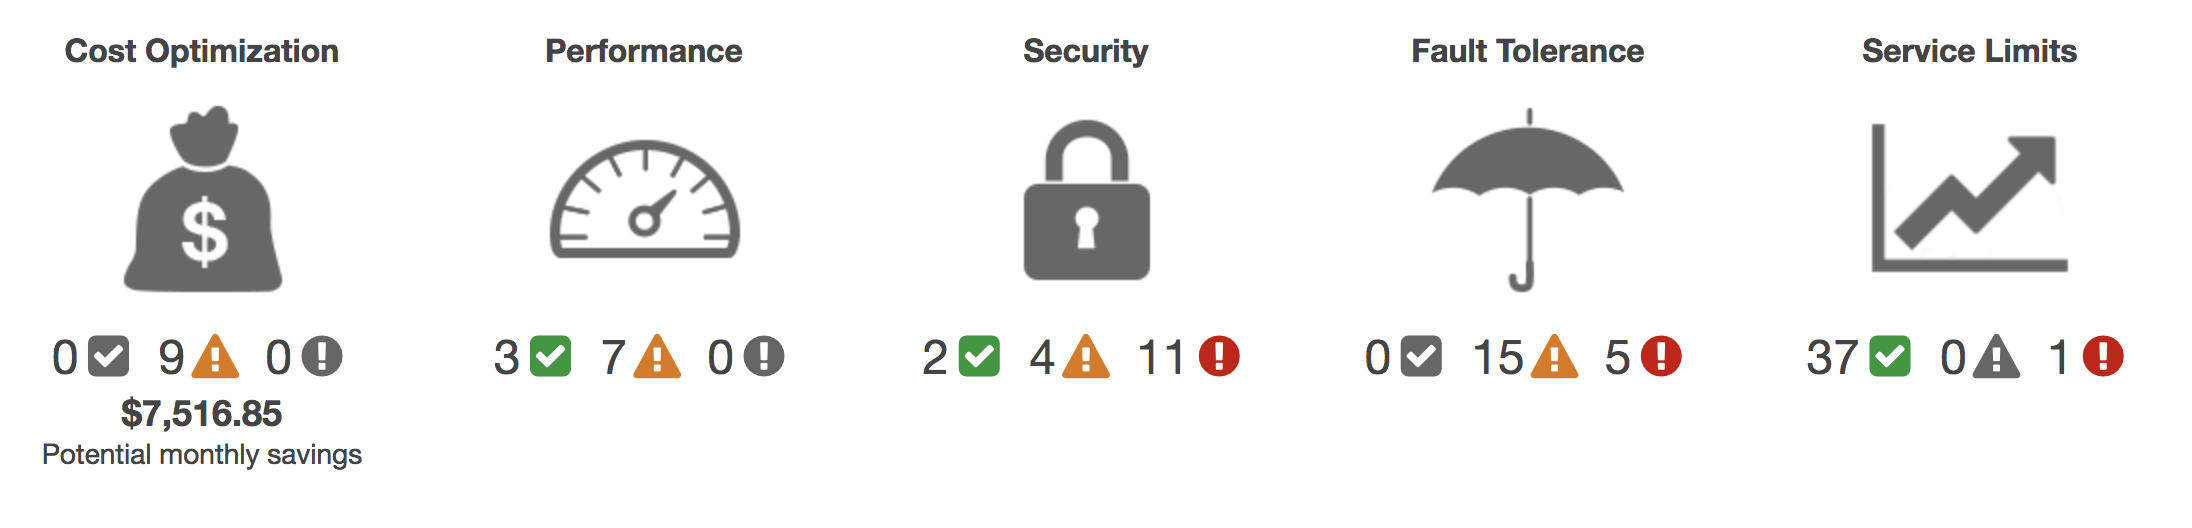
\includegraphics[scale=0.4]{sources/AWS_Trusted_Advisor_Kategorien}
      \caption[AWS Trusted Advisor Kategorien]{}
      \label{fig:AWS_Trusted_Advisor_Kategorien} AWS Trusted Advisor Kategorien
    \end{figure}

  Die \autoref{fig:AWS_Trusted_Advisor_Kategorien} zeigt die 5 Kategorien von Trusted Advisor mit jeweils 3 Arten von Indikatoren. 
  Die Indikatoren zeigen an, welche Prüfungen durchgeführt wurden.
  
  Grün bedeutet, dass keine Fehler oder zu prüfenden Empfehlungen vorhanden sind. Warnungen werden durch orangefarbene Indikatoren und Fehler durch rote Indikatoren angezeigt.
  
  Diese Empfehlungen sind eine Zusammenfassung auf hohem Niveau. Sie sind ein Startpunkt für die Untersuchung von Ressourcen mit Hilfe anderer Werkzeuge wie CloudWatch oder Cost-Explorer[ODER?].
\\\\

\textbf{Kostenoptimierung}\\
Die Empfehlungen zur Kostenoptimierung konzentrieren sich auf Möglichkeiten zur Kostensenkung, indem ungenutzte Ressourcen hervorgehoben werden. 
Sollten EC2-Instanzen mit geringer Auslastung gefunden werden, wird es diese bei Trusted Advisor signalisiert. Denn diese Instanzen verbrauchen Ressourcen und können terminiert oder pausiert werden. 
[HIER FEHLT...]
Auch nicht zugewiesene Elastic IP-Adressen erzeugen Kosten. Diese können gegebenenfalls von Trusted Advisor gefunden werden. %t.ly/nYiv
\\

\textbf{Leistungsgrenzen}\\
In dieser Kategorie werden Empfehlungen zur Vermeidung von Grenzwertüberschreitungen hervorgehoben.
Es wird zum Beispiel nach einer Nutzung gesucht, die mehr als 80 \% des Leistungsgrenzwerten für wichtige Dienste beträgt. Einige Beispiele sind  Amazon EC2, Auto Scaling, Elastic Block Store, Simple Email Service und AWS CloudFormation.
\\\\
Sich dieser Grenzen bewusst zu sein, gibt die Möglichkeit, rechtzeitig zu handeln und es trägt zu Kostenüberwachung bei.
[SAGEN OB DIESE GRENZE DIE GLEICHE WIE BEI CloudWatch SIND]
[ZEIGE BEISPIELE FueR Empfehlungen]\\
Bei der Erwägung von Trusted-Advisor ist zu überlegen, ob es kosteneffizient ist, für Pläne zu zahlen, die den Zugang zu allen Empfehlungen des Trusted Advisors ermöglichen. Das übergeordnete Ziel dieser Arbeit ist es, die Entstehung der Kosten auf eine praktikable Weise zu verstehen (Kostenüberwachung). Dies, um Optimierungsmaßnahmen zu ermöglichen. 
\\
Es wäre nicht sinnvoll, Kosten für Plänen wie Geschäfts- oder Enterprise Support zu übernehmen, wenn diese die möglichen Einsparungen übersteigen.  Die Vorteile von Geschäfts- oder Enterprise Support-Plänen beschränken sich nicht auf Kosteneinsparungen und Kostenbegrenzung, sondern tragen auch zur Sicherheit und Leistung bei. Jedes Unternehmen muss selbst entscheiden, ob es diese Informationen benötigt.
WIE TRIFFT MAN EINE ENTSCHEIDUNG IM UNTERNEHMEN? MODELLE?
\\
\subsection{Überwachungswerkzeuge gemäß ihrer Verwendung?}
\begin{figure}
  \centering
  \includegraphics[scale=0.6]{sources/ÜberwachungswerkzeugeNachVerwendung}
  \caption[Überwachungswerkzeuge gemäß ihrer Verwendung]{}
  \label{fig:ÜberwachungswerkzeugeNachVerwendung} Überwachungswerkzeuge gemäß ihrer Verwendung
\end{figure}

\textbf{Handlungsempfehlungen} \\
Überlegung 1: \\
Es kann in Erwägung gezogen werden, für einen begrenzten Zeitraum von 3 Monaten einen Support-Plan zu bezahlen, um aus den gegebenen Empfehlungen zu lernen. Oder Business-Plan alle 6 Monate für 1 Monat zu aktivieren.  
\\
Überlegung 2: \\ 
Ein Berater für eine Prüfung und Optimierung der Ressourcen kann in Deutschland zwischen x und b Dollar kosten. Dies ist nur eine Alternative zu den Plänen des Trusted-Advisor. Ein Berater, der alle 5 Kategorien abdeckt, könnte 555-999 kosten. Das sagt der Berater Juanito von der Firma XXX.
[WIE KANN ICH DIESE ÜBERLEGUNGEN RICHTIG DARSTELLEN?]
\\\\
\textbf{Summary/Fazit}\\
%[ABSCHLUSS DES KAPITELS/Überbrückung FÜR DAS KOMMENDE KAPITEL]}
% CloudWatch
In diesem Kapitel wurde gezeigt, wie es mit CloudWatch möglich ist, Alarme auf Basis von Ereignissen einzurichten, die mit Amazon SNS [IWO ERKLÄREN WAS DAS IST;Für Kommunikation innerhalb von AWS] oder externen E-Mail-Adressen kommunizieren. Im nächsten Kapitel wird CloudWatch erneut behandelt. Diesmal nicht als Überwachungswerkzeug, sondern als Optimierungswerkzeug zur Erstellung von automatisierte Aktionen/Reaktionen. Dazu war es notwendig, die Rolle der von CloudWatch gesammelten Metriken zu verstehen, die die Grundlage für die Verwaltung von Aktionen wie Auto-Scaling-Gruppen bilden. 
%Cost Explorer
Aus dem Blickwinkel des Kostenmanagements wurde gezeigt, wie man mit dem Cost-Explorer die Kosten der letzten 12 Monate analysieren, eine Einschätzung der Kosten im aktuellen Monat und eine Prognose für die nächsten Monate erhalten kann. Es ist möglich, die Kosten nach Tags und anderen Filtern zu trennen. Diese Informationen dient unter anderem zur Erstellung einer operativen Budgetplanung mit genaueren Daten.
%Trusted Advisor
Darüber hinaus wurde Trusted Advisor vorgestellt, die konkrete Optimierungsempfehlungen gibt und warnet über Leistungsgrenzen. Dies kann mit erheblichen Kosten verbunden sein und ist daher nicht für alle Arten von Unternehmen unmittelbar attraktiv. 
[WAS KOMMT IN NÄCHTEN KAP.?]

\begin{comment}
En este capitulo se  mostró de qué manera es posible con CloudWatch configurar alarmas basadas en eventos. Dichas alarmas comunican con Amazon SNS o direcciones de correo externas. En el capiulo siguiente se volverá a tematizar CloudWatch. Esta vez no como herramienta de monitoneo, sino de optimizacion para crear acciones ??? Para ello fue necesario entender que papel juegan las metricas recolectadas por CloudWatch, las cuales son la base para manejar los grupos Auto-Scaling. 

Desde la perspectiva del manejo de costos, se mostró como con Cost-Explorer es posible analizar los costos de los ultimos 12 meses, tener un calculo de los costos en el mes actual y recibir un pronostico de los proximos meses. Teniendo la posibilidad de separar los costos por medio de Tags y otros filtros. Dicha información contribuye a poder crear una planificacion de presupuestos operativa basada en datos de gran presicion.

Además se presentaron herramientas como Trusted Advisor las cuales brindan recomendaciones concretas sobre optimizacion y alertan si limites que se acercan a su umbral máximo. 

Este puede representar costos consideradable y que por lo tanto no lo hacen directamente atractivo para todo tipo de empresas. 
\end{comment}

\begin{comment}
AWS Cost Explorer Budgets show actual spend vs budget by month.
Filter by budgets, tags and tax, region, instances, usage type, cost category
Die Kosten vorhersehbar machen
Wiederverwendung gespeicherter Berichte. Welche Vorteile?

Da kann man sehen wie viele Stunden an RI und an On-Demand pro Tag/Monat verbraucht wurden.
-	Informationen um Schätzungen handelt, die von den tatsächlichen Kosten für den Abrechnungszeitraum abweichen können. %https://youtu.be/3peNAKB3VxA?t=705
-	Kann ich die Usage von S3 Einheiten und analysieren, wie häufig diese zugegriffen werden %https://youtu.be/pjrKDkzbas8?t=2425
-	Man könnte herausfinden, ob die RIs tatsächlich günstiger als ON-Demand sind. Wenn die RIs sind „konvertierbar“ und teurer als On-Demand, könnte man sich dafür entscheiden diese in was umzuwandeln, was genutzt wird. %https://youtu.be/pjrKDkzbas8?t=3385

%(How to use Spots and on-demand)
%detect CPU Utilization, with Amazon CloudWatch
\end{comment}
%IST taging EINE STRATEGIE?
%I could compute the cost of a query, user, transaction
% https://youtu.be/qYHR_V1lvNU?t=375